\documentclass[11pt, spanish]{article}
\usepackage[spanish]{babel}
\selectlanguage{spanish}
\usepackage[utf8]{inputenc}
\usepackage{amsmath}
\usepackage{amsfonts}
\usepackage{amsthm}
\usepackage{float}
\usepackage{graphicx}

% Margenes
\usepackage[left=2cm,right=2cm,top=2cm,bottom=1.5cm]{geometry}
%Espaciado
%\linespread{1.3}


\title{Introducción al Procesamiento Digital de Imágenes - Práctica 1}
\date{}

\begin{document}
\maketitle

Para preparar el entorno para poder ejecutar todos los programas,
primero debe tenerse instalado \texttt{python3} (y su \texttt{pip} correspondiente).
Luego, debe ejecutarse 
\begin{verbatim}
    virtualenv -p python3 venv 
    . venv/bin/activate
    pip install -r requirements.txt 
\end{verbatim}



\section{Ejercicio 1.a.}

La suma, la resta y el producto son las operaciones punto a punto
(o sea que requieren imágenes de las mismas dimensiones) y además saturan en 0 y 255
(con lo que las imágenes de producto serán generalmente muy claras).

Modo de uso
\begin{verbatim}
    python3 ej01-a.py <img1> <img2> <operacion>
\end{verbatim}


\begin{figure}[H]
\centering
  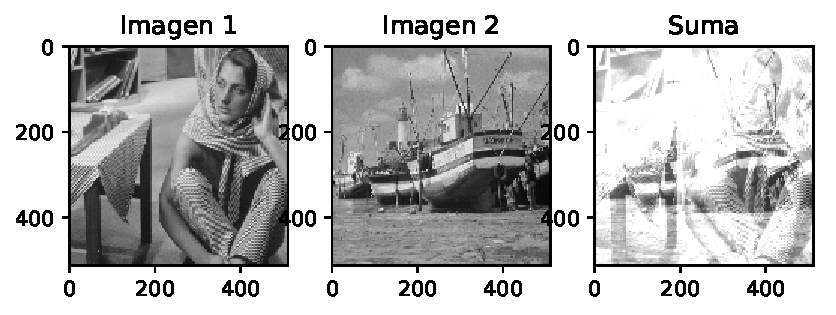
\includegraphics[height=6cm]{informe-imgs/ej01-a-suma.pdf}
  \caption{\texttt{python3 practica1/ej01-a.py barbara.png boat.png suma}}
\end{figure}

\begin{figure}[H]
\centering
  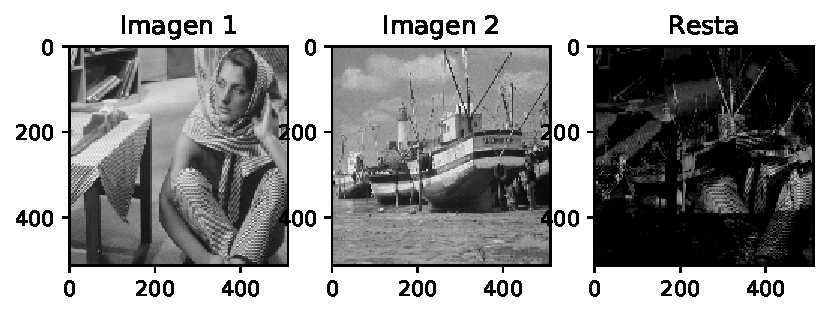
\includegraphics[height=6cm]{informe-imgs/ej01-a-resta.pdf}
  \caption{\texttt{python3 practica1/ej01-a.py barbara.png boat.png resta}}
\end{figure}

\begin{figure}[H]
\centering
  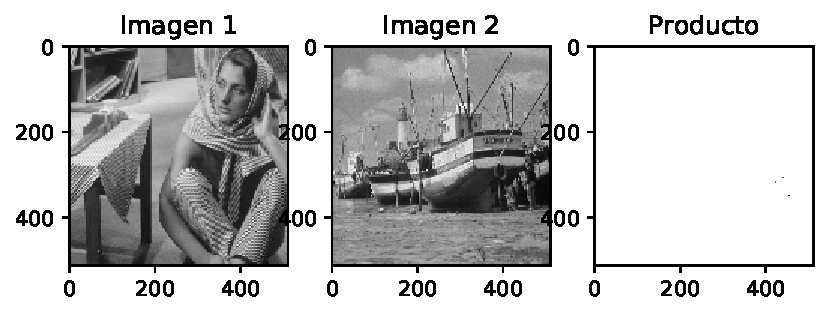
\includegraphics[height=6cm]{informe-imgs/ej01-a-producto.pdf}
  \caption{\texttt{python3 practica1/ej01-a.py barbara.png boat.png producto}}
\end{figure}


\section{Ejercicio 1.b.}

El producto por escalar es la operación punto a punto de multiplicar por un escalar, saturando en 255.

Modo de uso
\begin{verbatim}
    python3 ej01-b.py <img> <escalar>
\end{verbatim}


\begin{figure}[H]
\centering
  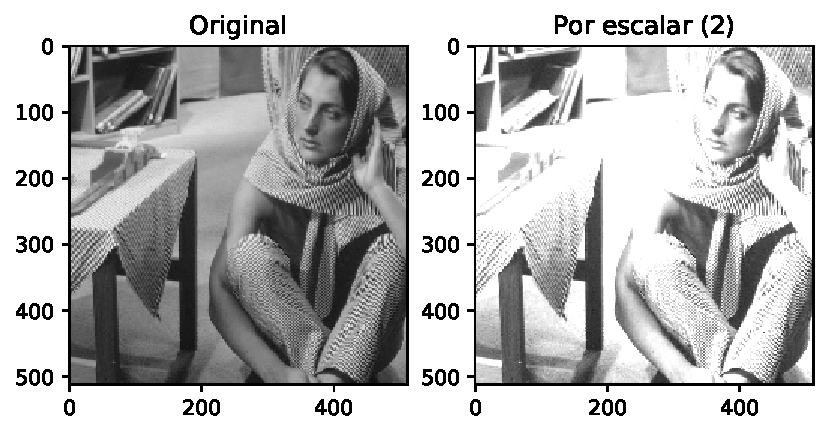
\includegraphics[height=6cm]{informe-imgs/ej01-b.pdf}
  \caption{\texttt{python3 practica1/ej01-b.py barbara.png 2}}
\end{figure}


\section{Ejercicio 1.c.}
Compresión de rango dinámico.

Modo de uso
\begin{verbatim}
    python3 ej01-c.py <img>
\end{verbatim}

\begin{figure}[H]
\centering
  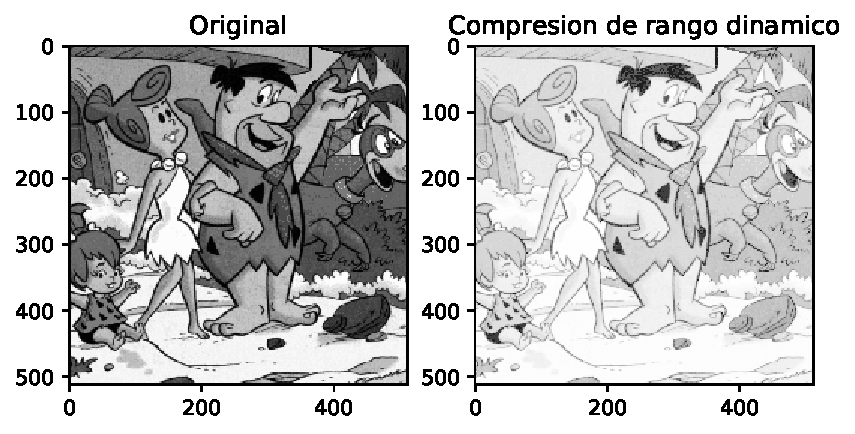
\includegraphics[height=6cm]{informe-imgs/ej01-c.pdf}
  \caption{\texttt{python3 practica1/ej01-c.py flintstones.png}}
\end{figure}


\section{Ejercicio 2.}
Negativo de una imagen.

Modo de uso
\begin{verbatim}
    python3 ej02.py <img>
\end{verbatim}

\begin{figure}[H]
\centering
  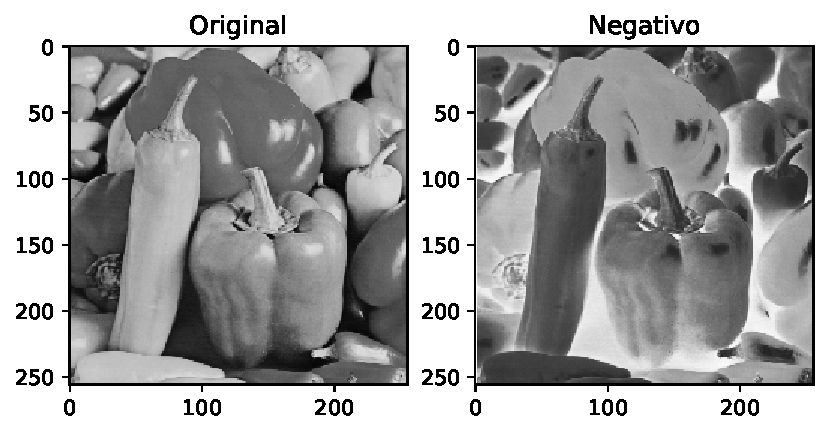
\includegraphics[height=6cm]{informe-imgs/ej02.pdf}
  \caption{\texttt{python3 practica1/ej02.py peppers256.png}}
\end{figure}


\section{Ejercicio 3.}
Todos los valores debajo de un umbral se transforman a negro.

Modo de uso
\begin{verbatim}
    python3 ej03.py <img> <umbral>
\end{verbatim}

\begin{figure}[H]
\centering
  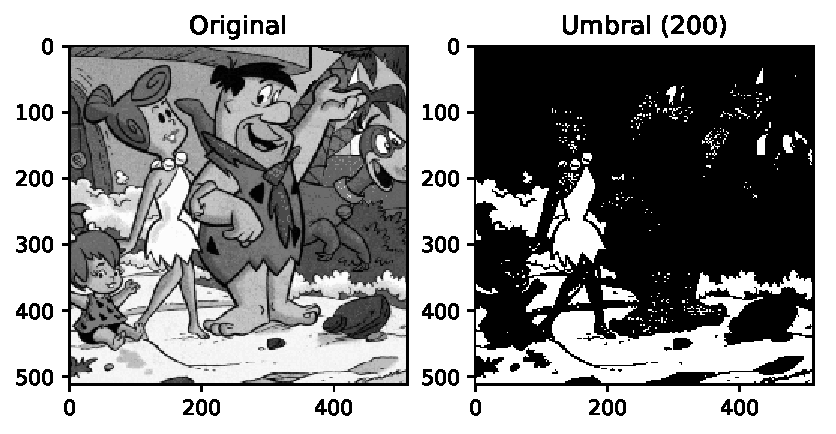
\includegraphics[height=6cm]{informe-imgs/ej03.pdf}
  \caption{\texttt{python3 practica1/ej03.py flintstones.png 200}}
\end{figure}


\section{Ejercicio 4.}
Fraccionamiento en planos de bits.

Modo de uso
\begin{verbatim}
    python3 ej04.py <img>
\end{verbatim}

\begin{figure}[H]
\centering
  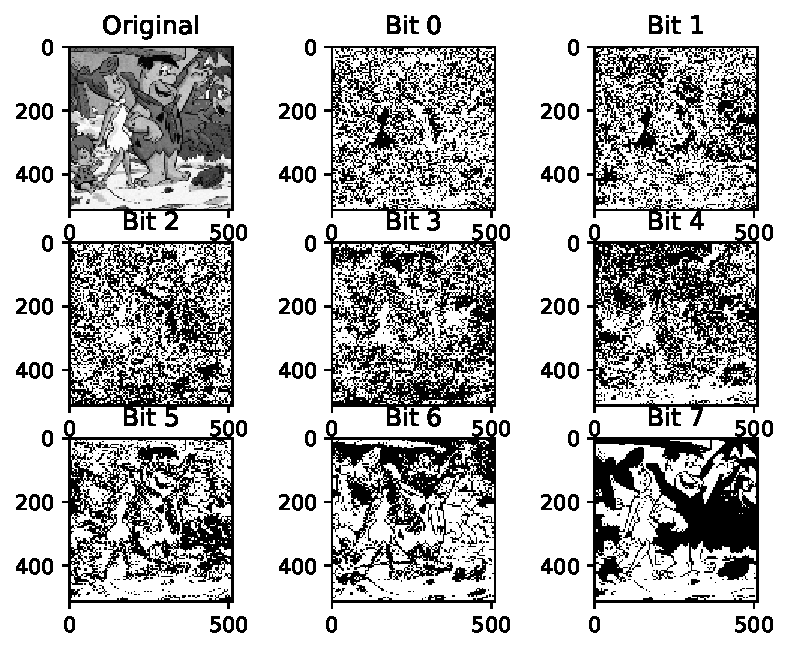
\includegraphics[width=1\textwidth]{informe-imgs/ej04.pdf}
  \caption{\texttt{python3 practica1/ej04.py flintstones.png}}
\end{figure}


\section{Ejercicio 5.}
Histogramas de una imagen. Muestra ambos el histograma y el histograma de la acumulada.

Modo de uso
\begin{verbatim}
    python3 ej05.py <img>
\end{verbatim}

\begin{figure}[H]
\centering
  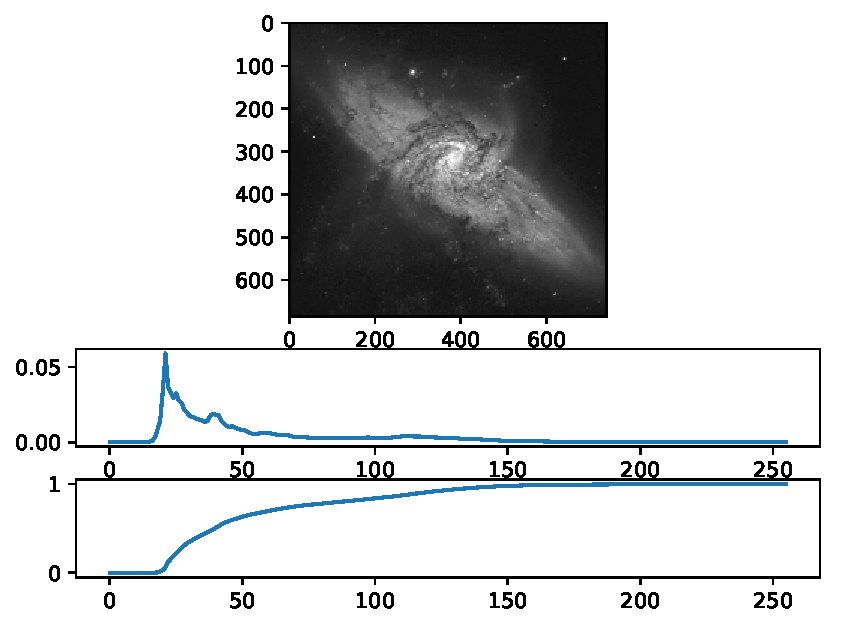
\includegraphics[width=6cm]{informe-imgs/ej05-1.pdf}
  \caption{\texttt{python3 practica1/ej05.py Fig30.jpg}}
\end{figure}

\begin{figure}[H]
\centering
  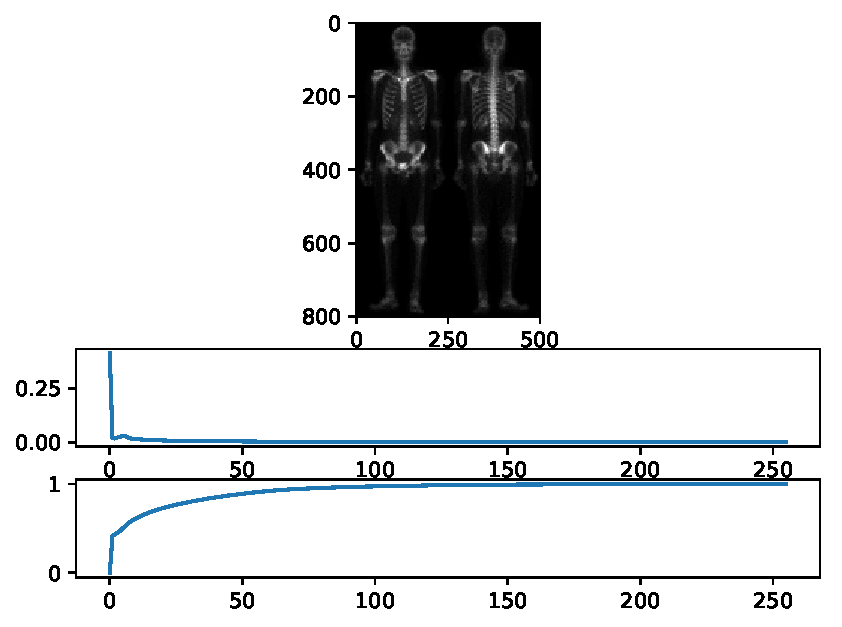
\includegraphics[width=6cm]{informe-imgs/ej05-2.pdf}
  \caption{\texttt{python3 practica1/ej05.py Fig46.jpg}}
\end{figure}

\end{document}

